In diesem Kapitel werden die Stärken und Schwächen des Unternehmens mit Fokus
auf den aktuellen Projektablauf genauer untersucht. Als Methode
wird die SWOT-Analyse\footnote{Die SWOT-Analyse ist ein Instrument um
Stärken, Schwächen, Chancen und Risiken darzustellen. Es eignet sich sowohl zur Situationsanalyse
wie auch als Instrument der Strategieformulierung. \citealp*[Vgl.][S. 134]{homburg2000quantitative}} 
verwendet und ist in der nachstehenden Grafik \ref{pic:swot_analyse} abgebildet.
Die einzelnen Punkte sind in Zusammenarbeit mit der Geschäftsleitung in einem Workshop
erarbeitet worden.

% Der Studierende ist sich bewusst, dass sich die Chancen und Risiken 
% nicht nur auf den Projektablauf sondern auf das ganze Unternehmen beziehen. 
% Da der Projektablauf jedoch ein Kernelement des Unternehmens ist, können sie 
% auch bei dieser Betrachtung verwendet werden.

\begin{figure}[htbp]
\begin{center}
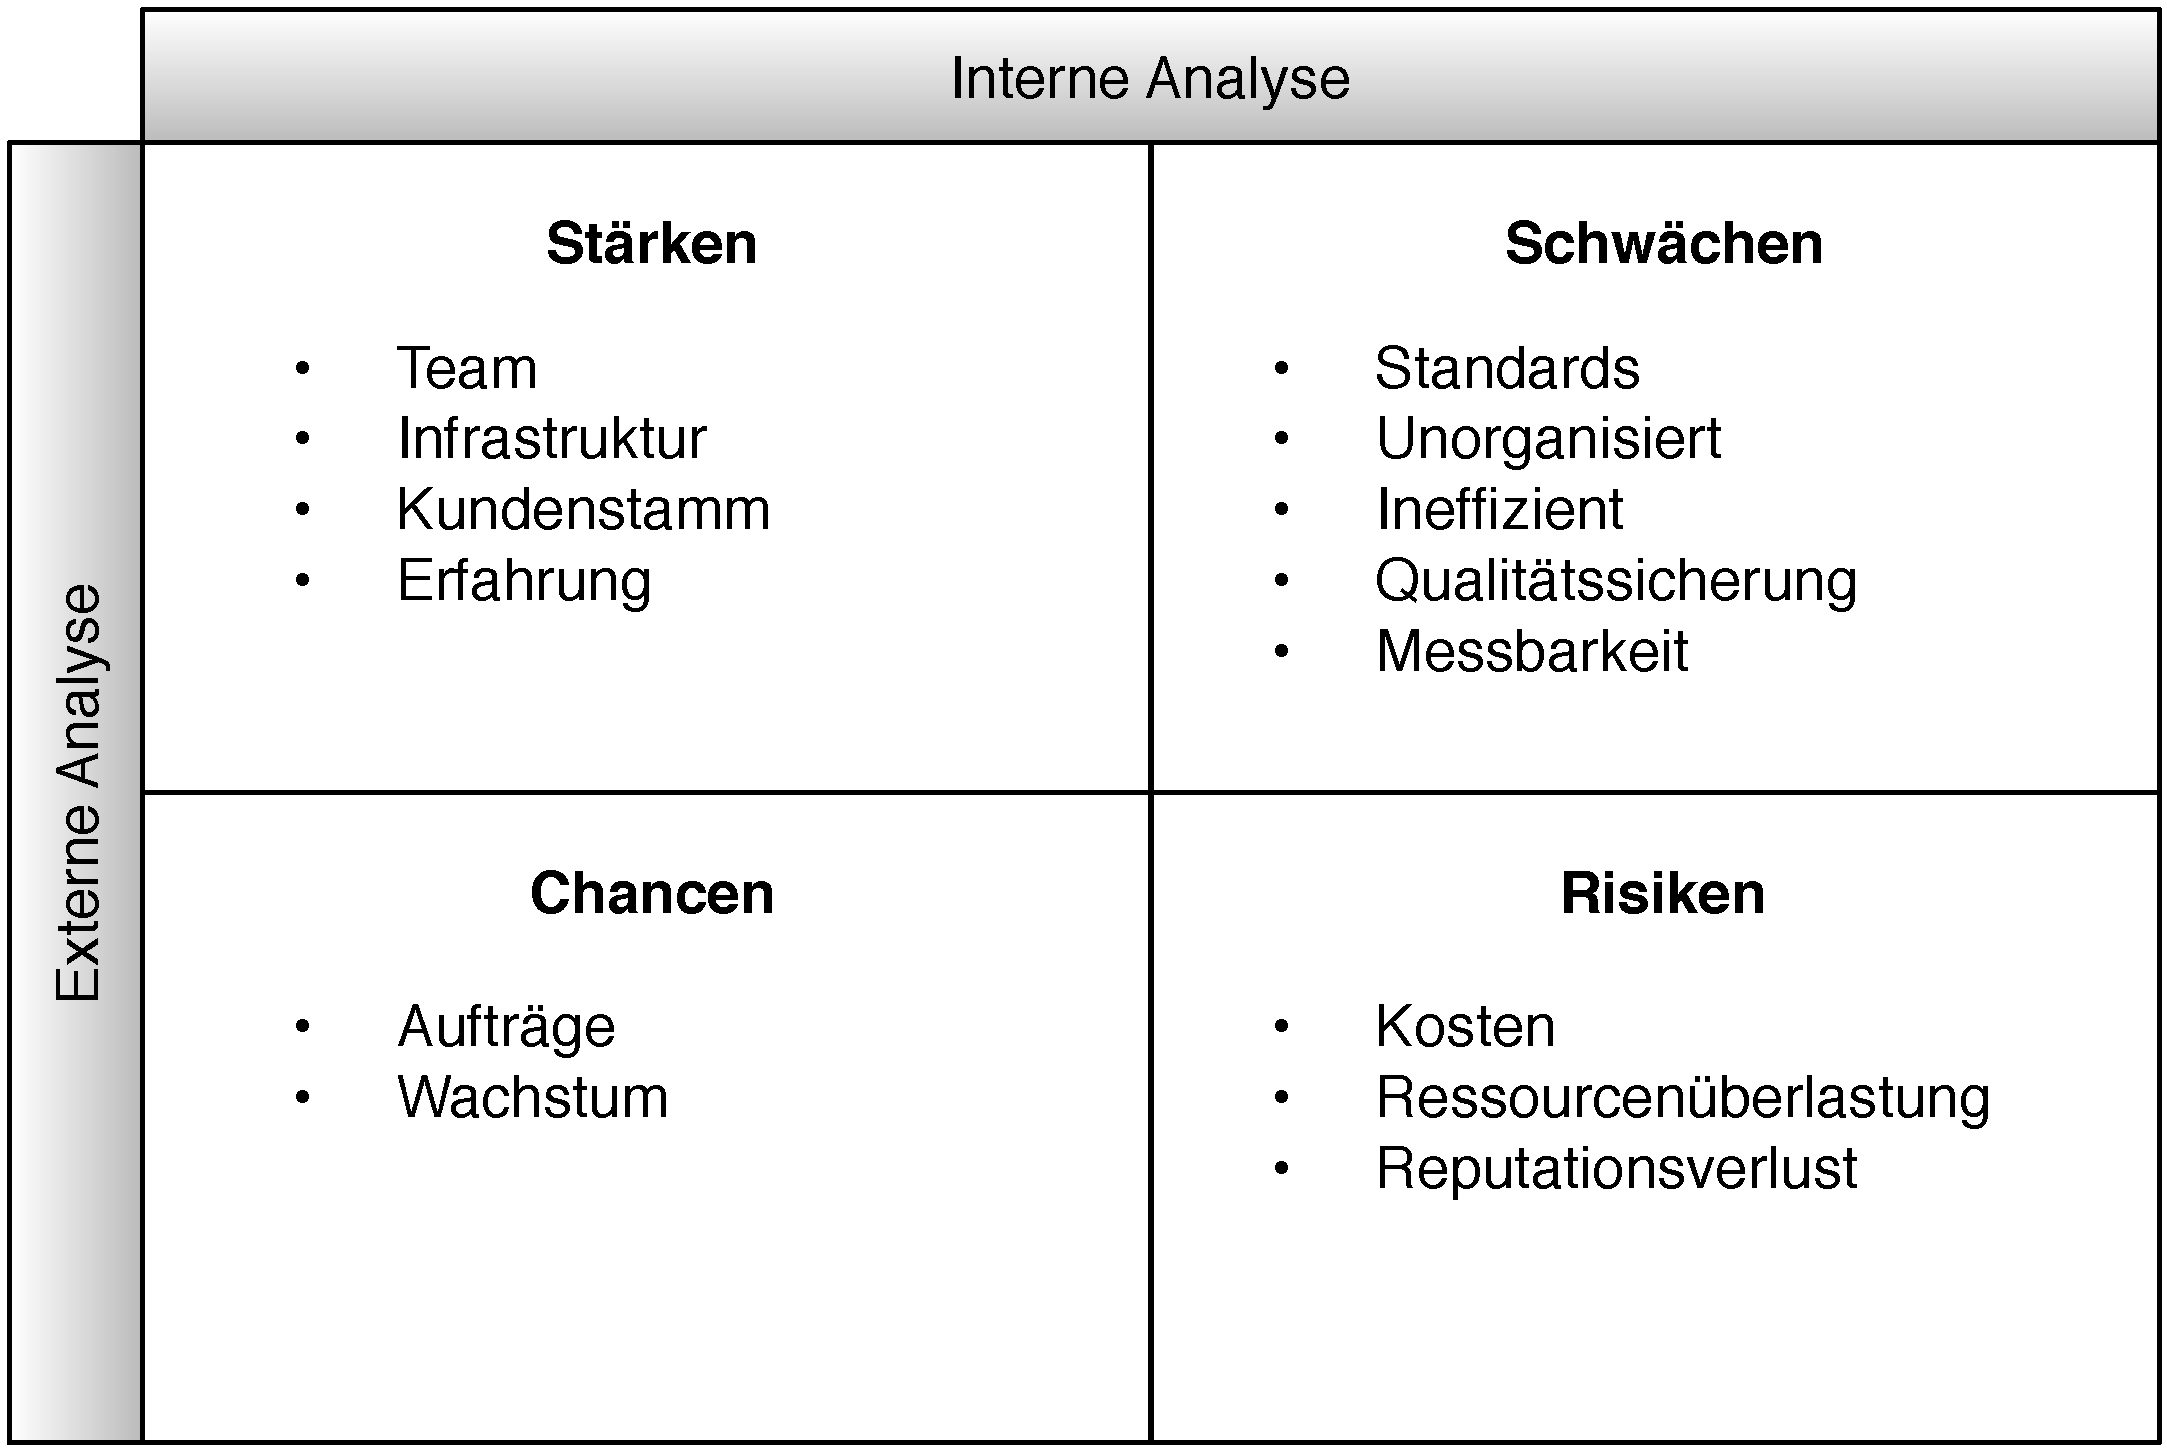
\includegraphics[width=0.8\textwidth,angle=0]{./bilder/analyse/swot_analyse.pdf}
\caption[SWOT-Analyse von allink]{SWOT-Analyse von allink\footnotemark}
\label{pic:swot_analyse}
\end{center}
\end{figure}
\footnotetext{Eigene Darstellung}

Es wird nun im Detail auf die einzelnen Punkte aus der SWOT-Analyse eingegangen
und wo möglich mit einem Beispiel aus der Praxis untermalt.

\subsection{Stärken}
Bei den Stärken handelt es sich um Eigenschaften des Unternehmens,
die es zu diesem Zeitpunkt mitbringt und teilweise noch nicht vollständig
ausnutzt. 

\subsubsection{Stabiles Team}
Das Unternehmen verfügt über ein starkes, ausgewogenes und interdisziplinäres Team. 
Sowohl im Bereich der Grafik wie auch der Informatik sind überaus fähige Mitarbeiter 
angestellt, deren Potenzial noch nicht vollständig ausgeschöpft wird. Die Beratung
befindet sich erst im Aufbau und das Unternehmen hat somit noch nicht ausreichend
Erfahrungen sammeln können. Die Mitarbeiter der Beratung sind ebenfalls
top motiviert, es ist jedoch noch zu früh um über die Fähigkeiten treffende
Aussagen machen zu können. Allgemein kann man das Team als extrem leistungswillig
bezeichnen, da sich alle zusammen mit der Agentur entwickeln möchten.

\subsubsection{Gute Infrastruktur}
Das Unternehmen verfügt über eine gute und moderne Infrastruktur. Kein Arbeitsgerät
ist älter als eineinhalb Jahre und überall sind die neusten Softwarepakete installiert.
Die allink legt grossen Wert auf gute Werkzeuge, da so die neusten Technologien
angewendet werden können und es daran nicht scheitern soll.

\subsubsection{Fundierte Erfahrung}
Durch die in den letzten fünf Jahren umgesetzten Projekte verfügt das Unternehmen
über einen grossen Erfahrungsschatz auf den es zurückgreifen kann. Das Hilft
überwiegend bei der Beratung von Kunden.
Auch verfügt das Unternehmen, wie man der Analyse der Kunden schon entnehmen
konnte, über einen relativ grossen Kundenstamm. Dies ist vor allem bei der
Akquisition sehr hilfreich, da man auf eine grosse Anzahl Referenzprojekte 
verweisen kann.

\subsection{Chancen}
Bei den Chancen handelt es sich um positive Auswirkungen, die zu erwarten sind,
wenn das Unternehmen die Schwächen in den Griff kriegt.

\subsubsection{Mehr Aufträge}
Der grosse Kundenstamm und die zur Zeit hohe Reputation des Unternehmens
birgt ein grosses Potenzial an neuen Aufträgen. Dabei ist das Potenzial der
Akquisition erst gering ausgeschöpft. Nur ein kleiner Prozentsatz der durchgeführten
Projekte in den letzten 5 Jahren wurde akquiriert. In den meisten Fällen entstanden
die Projekte durch direkte Anfragen von Kunden oder Partneragenturen.

\subsubsection{Gesundes Wachstum}
Die allink kann zur Zeit nicht alle Projektanfragen annehmen, da sie über zu
wenig Mitarbeiter verfügt. Es könnten mehr Mitarbeiter angestellt werden, dies
wurde aber bis anhin, durch die Anzeichen der Risiken die man schon mit dem bisherigen
Wachstum bewältigen muss, von der Geschäftsleitung vermieden.

\subsection{Schwächen}
Bei den Schwächen handelt es sich um Dinge die zur Zeit im Unternehmen nicht
optimal gelöst sind. Wenn diese nicht frühzeitig erkannt werden und nichts
dagegen unternommen wird, kann das die Entwicklung der Chancen verhindern und
das Eintreten der Risiken fördern.

\subsubsection{Fehlende Qualitätssicherung}
Durch die Überbelastung der Mitarbeiter können mit der Zeit die versprochenen Timings
nicht mehr eingehalten werden. Da die Ablagestrukturen nicht einheitlich geregelt
sind, kann es vorkommen, dass ein Mitarbeiter einem Kunden ein veraltetes oder
noch nicht freigegebenes Dokument sendet. Dies zieht einen zusätzlichen 
Mehraufwand mit sich, da man sich beim Kunden entschuldigen und rechtfertigen
muss. Zusätzlich strapaziert es auch die Beziehung zum Kunden.
Oft bleibt gegen Ende eines Projektes auch zu wenig Zeit die nötige 
Qualitätskontrollen durchzuführen, da man sich möglichst schnell um ein anderes,
möglicherweise auch schon überfälliges, Projekt kümmern muss. Der Kunde entdeckt
dann offensichtliche Fehler selbst und zweifelt zwangsläufig an der ganzen Arbeit.

\subsubsection{Mangelnde Effizienz}
Einfache Abläufe werden unnötig verkompliziert. Daten von vergangenen Projekten 
sind nicht mehr auffindbar, da sie nicht sauber archiviert wurden. Die ganze
Struktur wird dadurch langsam und ineffizient. Was sich wiederum negativ auf die zur
Verfügung stehende Zeit auswirkt.
Man hält zudem vor, während und nach einem Projekt nur an wenigen Standards fest. 
Das ganze Vorgehen ist nicht einheitlich, da in jedem Projekt wieder von
neuem entschieden wird, wie man vorgehen will. Es werden nur wenige einheitliche
Dokumente verwendet, zum Beispiel für die Erstellung von Offerten und Rechnungen.
Aber auch da entstehen schnell Fehler, zum Beispiel während der Umstellungen des 
Mehrwert Steuersatzes von 7.6\% auf 8\%. Da kein einheitliches Basistemplate
existiert, muss bei jeder Rechnung noch einmal sichergestellten werden, dass
der korrekte Steuersatz hinterlegt ist.

\subsubsection{Kein Controlling}
Auch bietet die fehlende bzw. chaotische Struktur nur wenige Punkte um Kennzahlen
zu messen. Den Umsatz den man mit dem Projekt erzielt hat ist zwar bekannt,
jedoch kann nur aus dem Gefühl heraus erahnt werden, ob mit dem Projekt einen
Gewinn für die Firma erzielt werden konnte. Die Mitarbeiter sind zwar angehalten
ihre Stunden in ein gemeinsames Stundenwidget einzutragen, jedoch werden
die Informationen nicht ausgewertet und können nicht mehr einzelnen Mitarbeitern
zugeordnet werden.

\subsection{Risiken}
Bei den Risiken handelt es sich um negative Auswirkungen, die zu erwarten sind,
wenn das Unternehmen die Schwächen nicht in den Griff bekommt.

\subsubsection{Hohe Kosten}
Durch die fehlende Kontrolle während eines Projektes, verliert man die
Übersicht über die Aufwände und schlussendlich die Kosten. Dadurch entsteht
ein Kostenrisiko, welches Konsequenzen für die Liquidität von allink haben kann.

\subsubsection{Ressourcenüberlastung}
Die Belastung für den Mitarbeiter wie auch für die Partner ist so über
längere Zeit nicht tragbar. Durch eine Überarbeitung kann es zu Ausfällen kommen, die
die Situation zusätzlich verschlimmern könnten. Das ganze Endet in einer 
schlechten Firmenkultur und das Unternehmung beginnt von Innen zu zerfallen.

\subsubsection{Reputationsverlust}
Da man Timings nicht mehr einhalten kann und man sich gegenüber dem Kunden
oft rechtfertigen muss entsteht ein schlechtes Bild der Unternehmung und sie
verliert an Vertrauen. Da die Konkurrenz im Tätigkeitsfeld der allink relativ
gross ist, ist ein möglicher Absprung und Angenturwechsel seitens des Kunden nicht 
auszuschliessen.
